% Previous work into shearing bijels have demonstrated how particles prefer to move in the direction of shear and if strong enough, even detach from the interface. \cite{bonaccorso_shear_2020} It has also been shown how at curved interfaces, ellipsoidal particles  

\section{Introduction}

While the microstructure and synthesis techniques for bijels have been explored in earnest, the rheology of bijels
has only recently seen an uptick in interest. Some interesting phenomena for bijels and shearing include the 
presence of monogels, made by remixing the phase separated liquid domains of the bijel while the electrostatic
interactions between particles maintains the structure of the particle monolayer. \cite{sanz_colloidal_2009} 
This behavior is system specific, suggesting the fluid system plays a role in this behavior as well. \cite{tavacoli_novel_2011}
\cite{bai_dynamics_2015} Investigations have identified that confined bijels under shear undergo elongation of
the domains in the direction of shear succeeded by particle detachment from the interface and eventual failure of the bijel. \cite{bonaccorso_shear_2020}
More recently, bijels have been identified to be 2D glasses percolating in 3D space, characterized through comparing the complex rheology of bijels against
colloidal gels made from silica particles with electrostatic interactions. \cite{ching_bijel_2022} 

In many of the manufacturing techniques outlined for continuous bijel production such as STrIPS, the rheological properties are essential in ensuring that 
the casting mixture remains processable. \cite{haase_continuous_2015,haase_situ_2016} While particle stabilized emulsions have been shown to be shear thinning, 
our investigation into magnetically stimuli responsive bijels will modify the behavior of these systems due to the application of magnetic fields. Past work with 
ferrofluids and magnetic emulsions have showed how the rheological properties vary drastically as a function of the field strength due to the orientation of the 
particles. \cite{qiao_magnetorheological_2012} The orientation of the particle to shear as well as the nematic order of particles 
can cause shear banding and a smaller effective viscosity owing to a smaller cross sectional area being presented to the direction of shear. 

In this chapter, we probe the dynamics of bijels under constant and complex shear to understand how the application of magnetic fields onto bijels stabilized with
anisotropic particles. We define a shear capillary number $Ca_s = \frac{\eta_{f} \dot{\gamma} L_{1}}{\sigma}$ where $\dot{\gamma} = \frac{2u_{LE}}{L_x}$ is the
strain rate and $L_1$ is the average domain size. \cite{frijters_effects_2012, yang_capillary_2022} In the literature, $Ca_s$ has been between between 0.04 
and 0.16. However, the box size in these simulations were smaller, meaning that these capillary number ranges would exceed the 
maximum mach number the model allows if this same range were used $(Ma \leq 0.03)$. To accommodate this limitation the 
largest capillary number used will be $Ca_s = 10^-5$ which correspond to a maximum of $Ma \approx 0.002$. $Ca_s = 10^-6,  
10^-7$ will also be used to demonstrate how the bijels respond to shear of varying strengths. As all particles used 
have only hard-sphere type interactions, it is expected that the behaviour seen should mimic 2D colloidal glasses 
percolating in 3D space, akin to what Ching and Mohraz saw, with an additional dependence on -the direction of shear. 
This would predict the discovery of particle monolayer dependent elasticity and yield stress along with shear thinning 
behaviour as a function of strain rate. 

To verify these predictions, bijel microstructure will be defined using four processing histories; The first is of a 
bijel simulated under a $\Bar{B} = 1$ magnetic field strength, the second is a bijel stimulated under no field, 
followed by the application of a $\Bar{B} = 1$ field after jamming, the third is a bijel simulated under no field, 
while the final microstructure is a bijel simulated under $\Bar{B} = 1$ magnetic field, followed by switching the 
field off after jamming. This gives insight into the impact of processing history on the shear properties of a bijel, 
in addition to the microstructural and colloidal insights gained. Based on the results in Bonaccorso et al., there 
should be shear driven and shear rate dependent elongation of the domains in the direction parallel to the applied 
shear which in this system will be seen as a reduction in $L_{\perp}$ and an increase in $L_{\parallel}$. 
\cite{bonaccorso_shear_2020} The microstructure anisotropy will also be a factor in the viscosity results, as 
larger domains are more permeable than smaller ones, meaning that bijels where $L_{\perp} > L_{\parallel}$ should 
see less of the domain elongation effects shown in Bonaccorso et al. as the permeability of the bijels rises with 
larger domain size. \cite{bonaccorso_shear_2020}

It is also expected that the effective viscosity will be different between the four microstructures dependent upon the 
degree of nematic ordering and microstructural anisotropy of the bijel. Nematic ordering of the particles will be mimic 
shear banding in colloidal suspensions, resulting in a lowered effective viscosity compared to bijels without nematically 
ordered particles. \cite{xu_relation_2013, vermant_flow-induced_2005} Tracking of the proportion of particles on the 
interface will also yield insight into how the packing of the particles affects the rate at which particles will get 
ejected from the interface. Systems with a larger $\eta_{eff}$ are predicted to have the largest domains, largest 
difference between initial and final particle order and lowest number of particles left on the interface once steady 
state has been established. 

We begin our investigation by analyzing the domain size change over time for bijels stabilized by ellipsoidal particles. We also
focus our attention on the effect of the initial state of the particle monolayer, in addition to the addition or removal of magnetic
fields. We perform this analysis on bijels stabilized by oblate and prolate particles. Bijel templates simulated in Aim 1 with no
field and a field strength of $\bar{B} = 1$ stabilized with a particle volume fraction $\phi_p = 0.15$. We apply a field strength of
$\bar{B} = 1$ or switch off the applied field. This results in four setups, $\bar{B}:0\rightarrow 0$, $\bar{B}:0\rightarrow 1$,
$\bar{B}:1\rightarrow 0$ and $\bar{B}:1\rightarrow 1$. We then define a shear capillary number, 
$Ca_s = \frac{\dot{\gamma} R_{s} \eta_{f}}{\sigma}$ where $\dot{\gamma}$ is the applied strain rate, $R_s$ is the equivalent
spherical radius of the particles, $R_s = 7.9$, $\eta_f$ is the dynamic viscosity of the fluid and $\sigma$ is the surface tension
of the interface. We use five shear numbers, $Ca_s = 1\cdot10^{-4}, 5\cdot10^{-5}, 1\cdot10^{-5}, 5\cdot10^{-6}, 1\cdot10^{-6}$.

\section{Results}\label{sec:results_p3}
\subsection{Microstructure change}

First we plot the domain size of each system over time to analyze the effect of application of shear and magnetic fields.

\begin{figure} 
    \centering 
    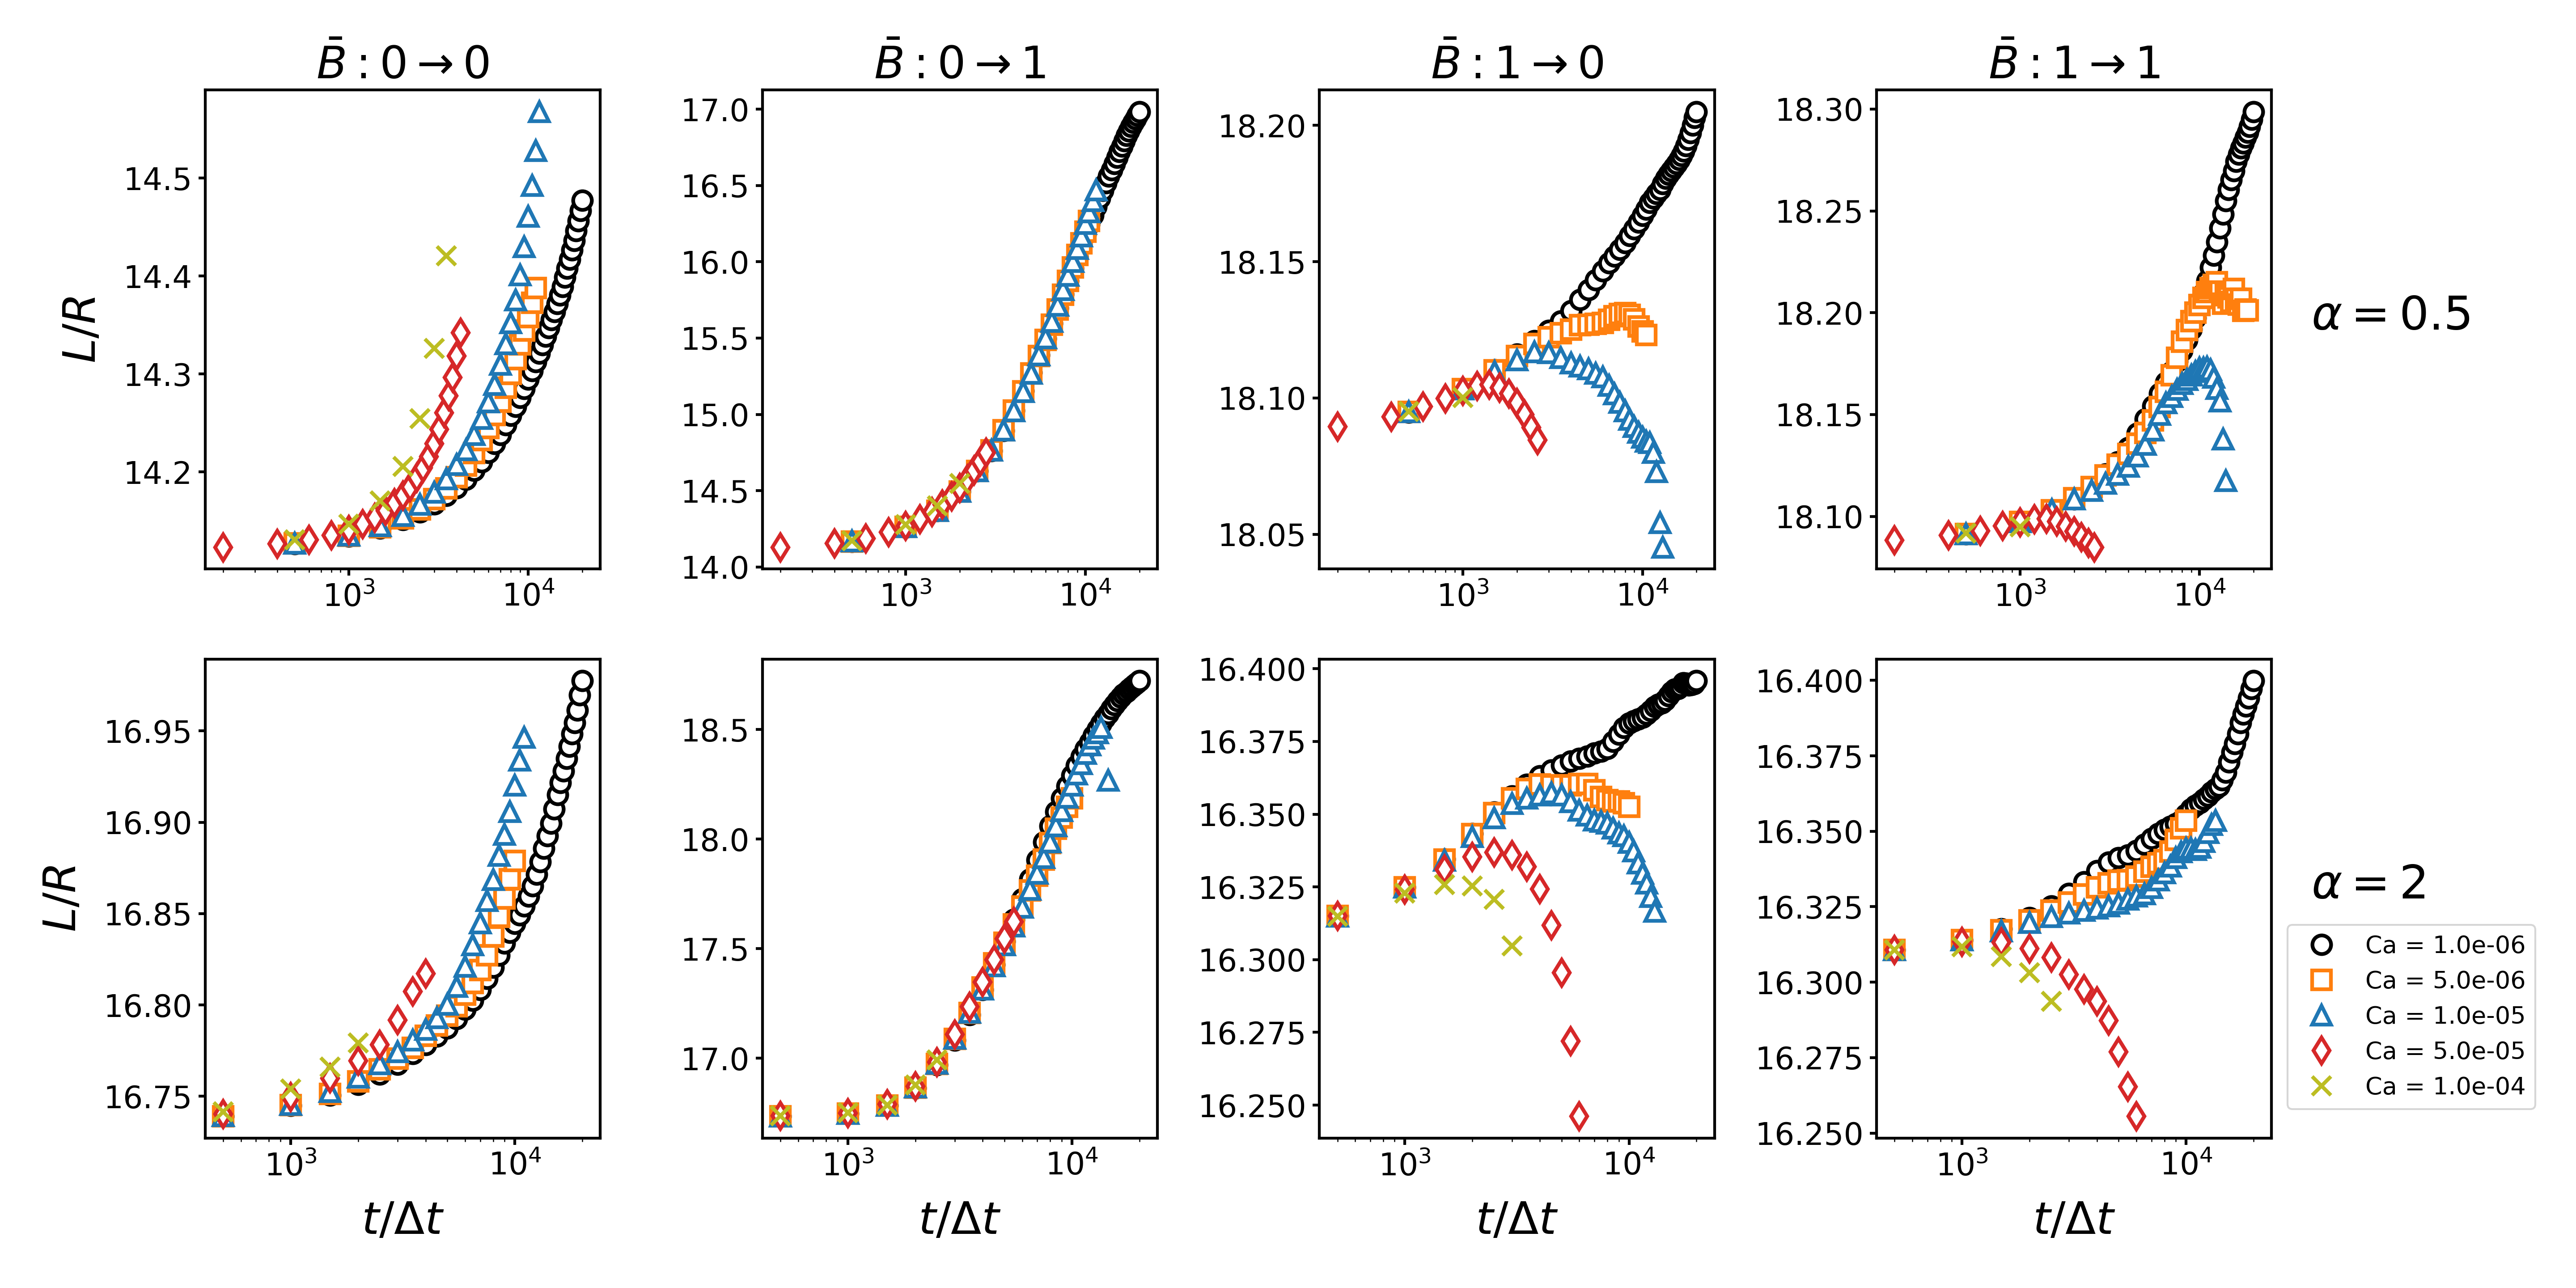
\includegraphics[scale=0.3]{../figures/results/paper3/domain_size-time_compare.png} 
    \caption{Comparisons of the time evolution of the average domain size for bijels stabilized by ellipsoidal particles undergoing
             various shear rates under four processes. Initially, the domain size coarsens for all runs under applied shear before
             reducing in some cases.} 
    \label{fig:domain_size_time_shear} 
\end{figure}

From Figure \ref{fig:domain_size_time_shear}, domains generally coarsen with time but the presence of a magnetic field 
significantly alters the coarsening dynamics due to magnetic field driven particle reordering on the interface. In the 
$\bar{B}: 1 \to 0$ and $\bar{B}: 1 \to 1$ cases, an initial plateau in domain size is observed, followed by a divergence in 
growth depending on $Ca$. The shear rate appears to influence domain coarsening, with higher $Ca_s$ leading to delayed or 
suppressed growth, especially in the presence of a field. The difference between applying $\bar{B}: 0 \to 1$ and 
removing $\bar{B}: 1 \to 0$ the field demonstrates the stability of the particle monolayer when a field is switched off.
There is little difference in the qualitative trends of domain size change for bijels stabilized with oblate or prolate particles,
This analysis highlights how the interplay between shear, capillary effects, and magnetic interactions governs bijel 
microstructural stability and evolution, offering insights into tunable bijel design for applications requiring controlled 
domain morphology. Domain coarsening   

\begin{figure} 
    \centering 
    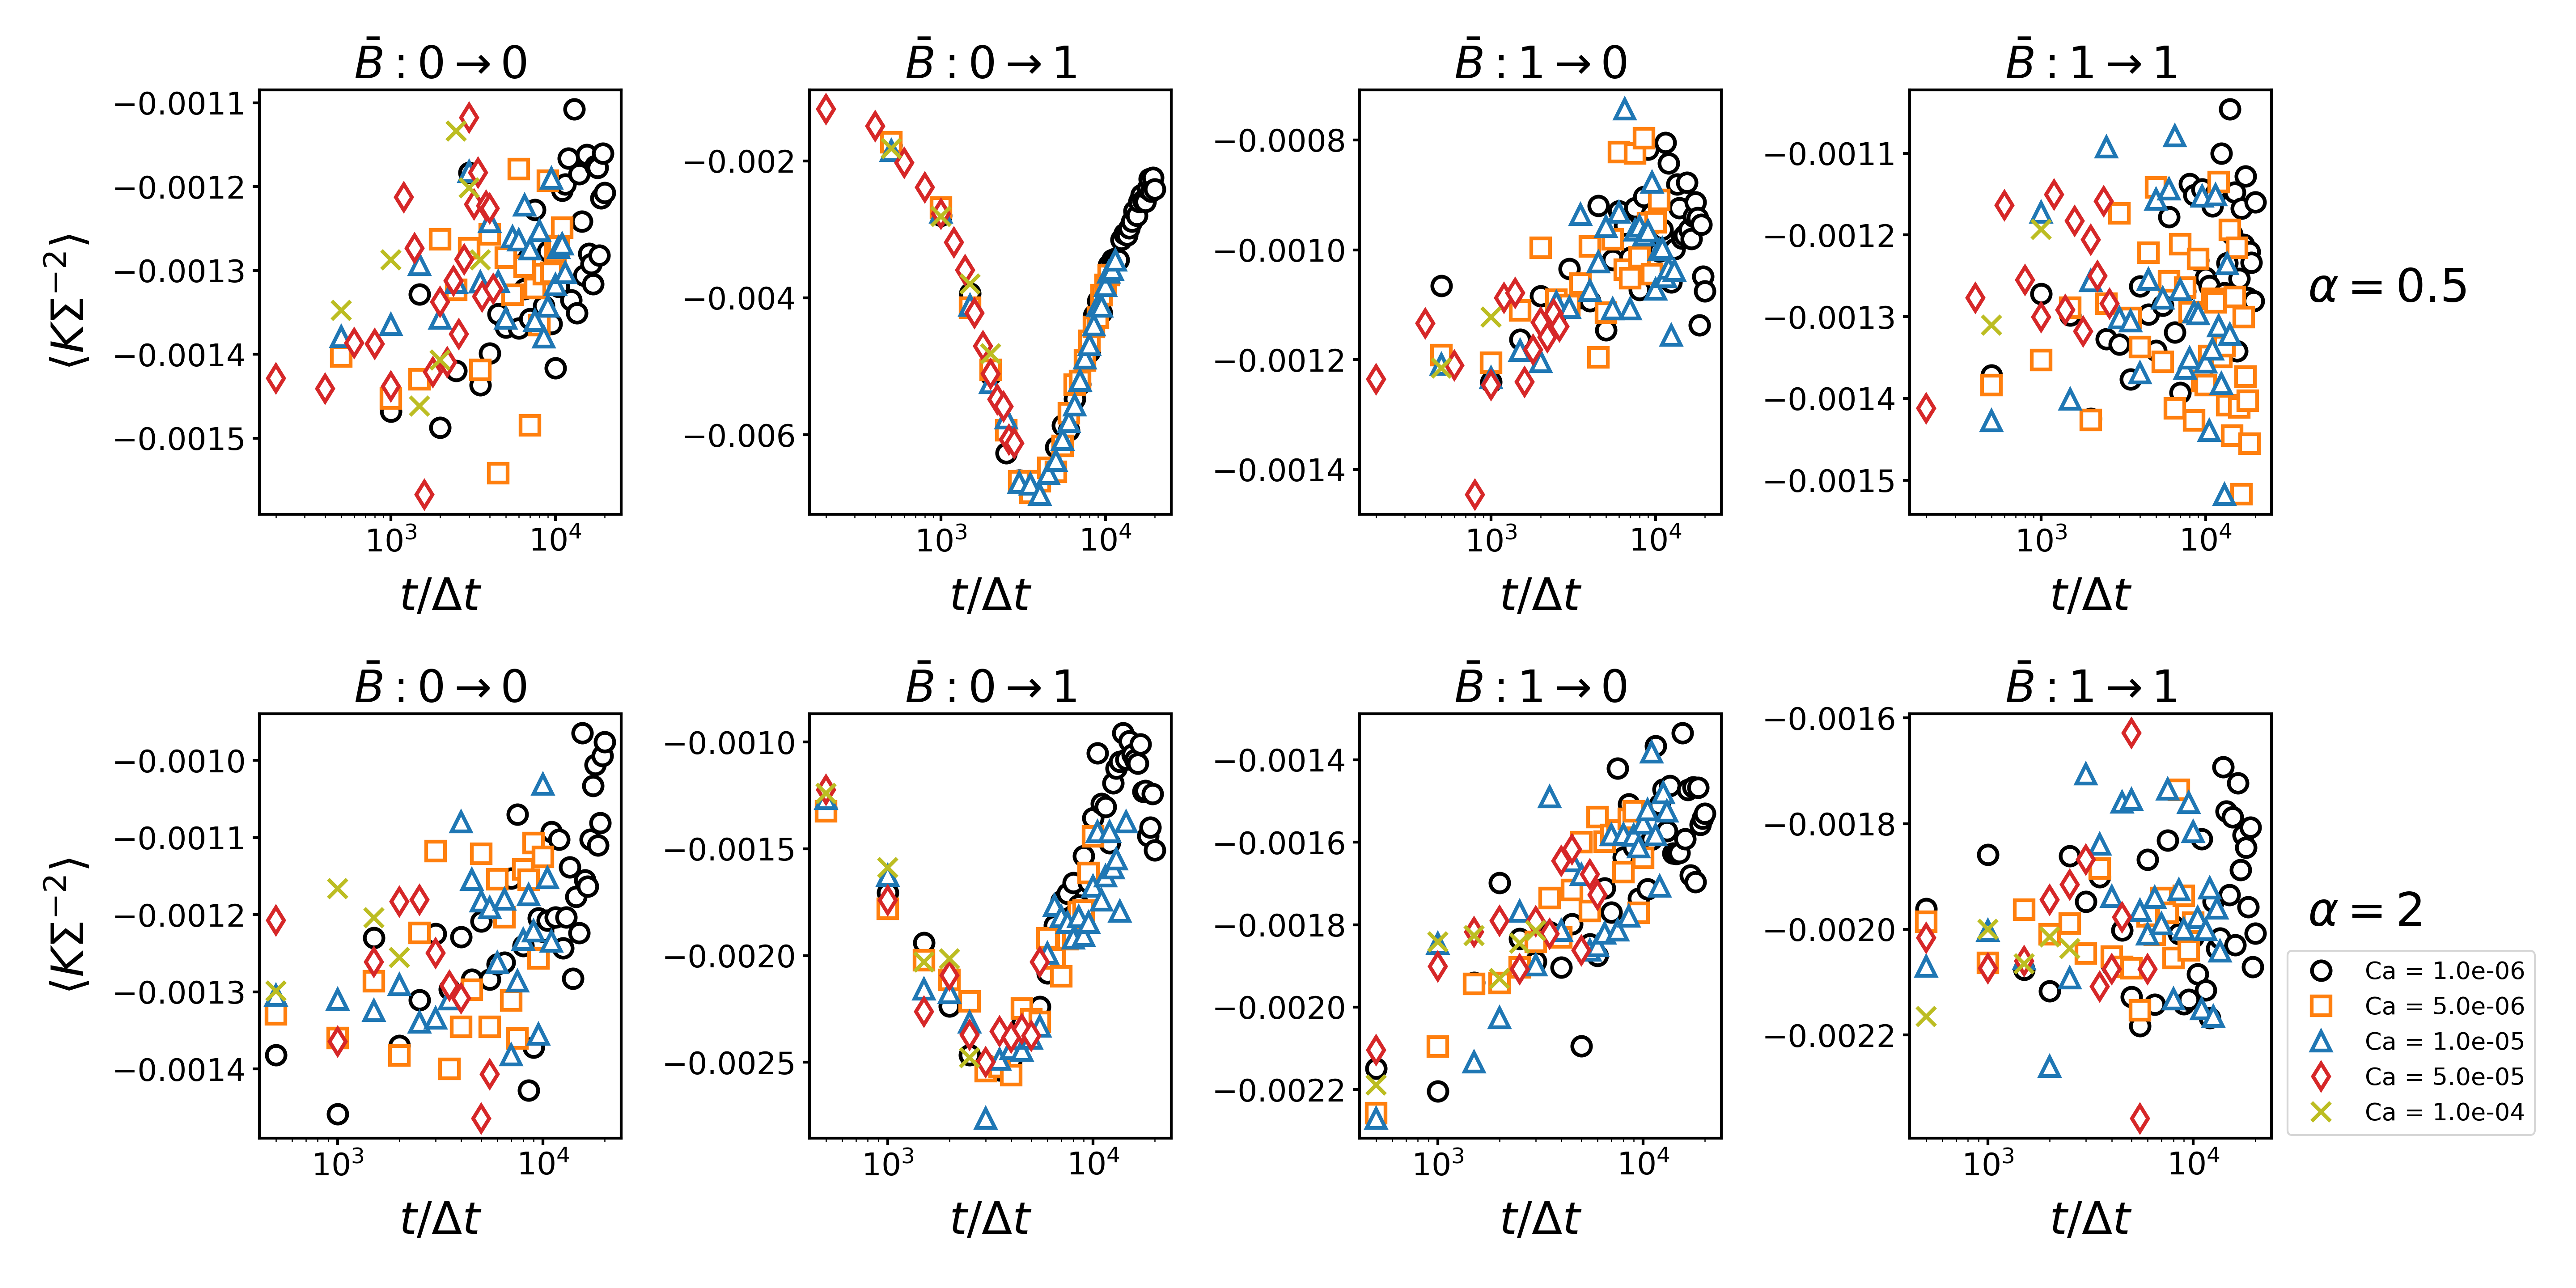
\includegraphics[scale=0.3]{../figures/results/paper3/gaussian-time_compare.png} 
    \caption{Plots of the time evolution of the area averaged Gaussian curvature $\langle K \Sigma^{-2} \rangle$ for four 
             processing histories applied to bijels stabilized with oblate and prolate ellipsoids. We demonstrate that the 
             magnitude of the gaussian curvature reduces for all systems except for $\bar{B}: 0 \to 1$.} 
    \label{fig:gaussian_curvature_time_shear} 
\end{figure}

Figure \ref{fig:gaussian_curvature_time_shear} reveals that the area averaged Gaussian curvature generally decreases in magnitude over time for all cases except 
$\bar{B}: 0 \to 1$. We also characterize that the curvature evolution of all systems are shear independent. $\bar{B}: 0 \to 1$ is
unique because particle rearrangements at the interface dominates the dynamics of the microstructure, not observed in all other
cases. From the time evolution of the curvature, we show that the same mechanism drives domain coarsening in all cases. Domain
coarsening is driven through a reduction in the interfacial area covered by the particle monolayer. Previous investigates have 
demonstrated how the orientation and arrangement of particles on the interface affect the domain size. 
\cite{gunther_timescales_2014} We focus our investigation on this aspect in the following section. 

\subsection{Particle properties}

Particles at the interface of bijels stabilized with ellipsoidal particles reorient at the interface to minimize interfacial and
steric energies. \cite{gunther_timescales_2014} The particles stabilizing bijels in confined systems under shear have been shown to
orient to the direction of shear and ejected from the interface at sufficiently long times or shear.\cite{bonaccorso_shear_2020} 
We probe these aspects of the particle monolayer in this section.

\begin{figure} 
    \centering 
    \includegraphics[scale=0.3]{../figures/results/paper3/angle_to_cartesian-SS.png} 
    \caption{Comparisons of the initial and final particle orientations of the particles to each cartesian direction under
             four processing histories for bijels stabilized with oblate and prolate ellipsoids at multiple shear rates. We show
             shear dependent ordering of the particle monolayer if the initial particle monolayer begins with particle order.} 
    \label{fig:particle_orientation_cartesian_shear} 
\end{figure}

From Figure \ref{fig:particle_orientation_cartesian_shear} we see that with bijel templates simulated under $\bar{B} = 0$, the
particles adopt a random orientation. Upon application of shear, we see that there is little directional ordering to the 
shear direction. Upon application of the magnetic field, the particle order to the direction of the magnetic field. When 
investigating the orientational ordering of a bijel simulated under a field strength of $\bar{B} = 1$, we see that there is
shear dependent decay of the orientational ordering when the magnetic field is removed. We also characterize similar behavior
when maintaining the applied field, indicating that two reasons for surface area reduction is present. These mechanisms are attributed
to reorientation of particles at the interface or ejection of particles from the interface. We can characterize the former mechanism
using the average interfacial angle between the particle and the interface $\langle \psi \rangle$.

\begin{figure} 
    \centering 
    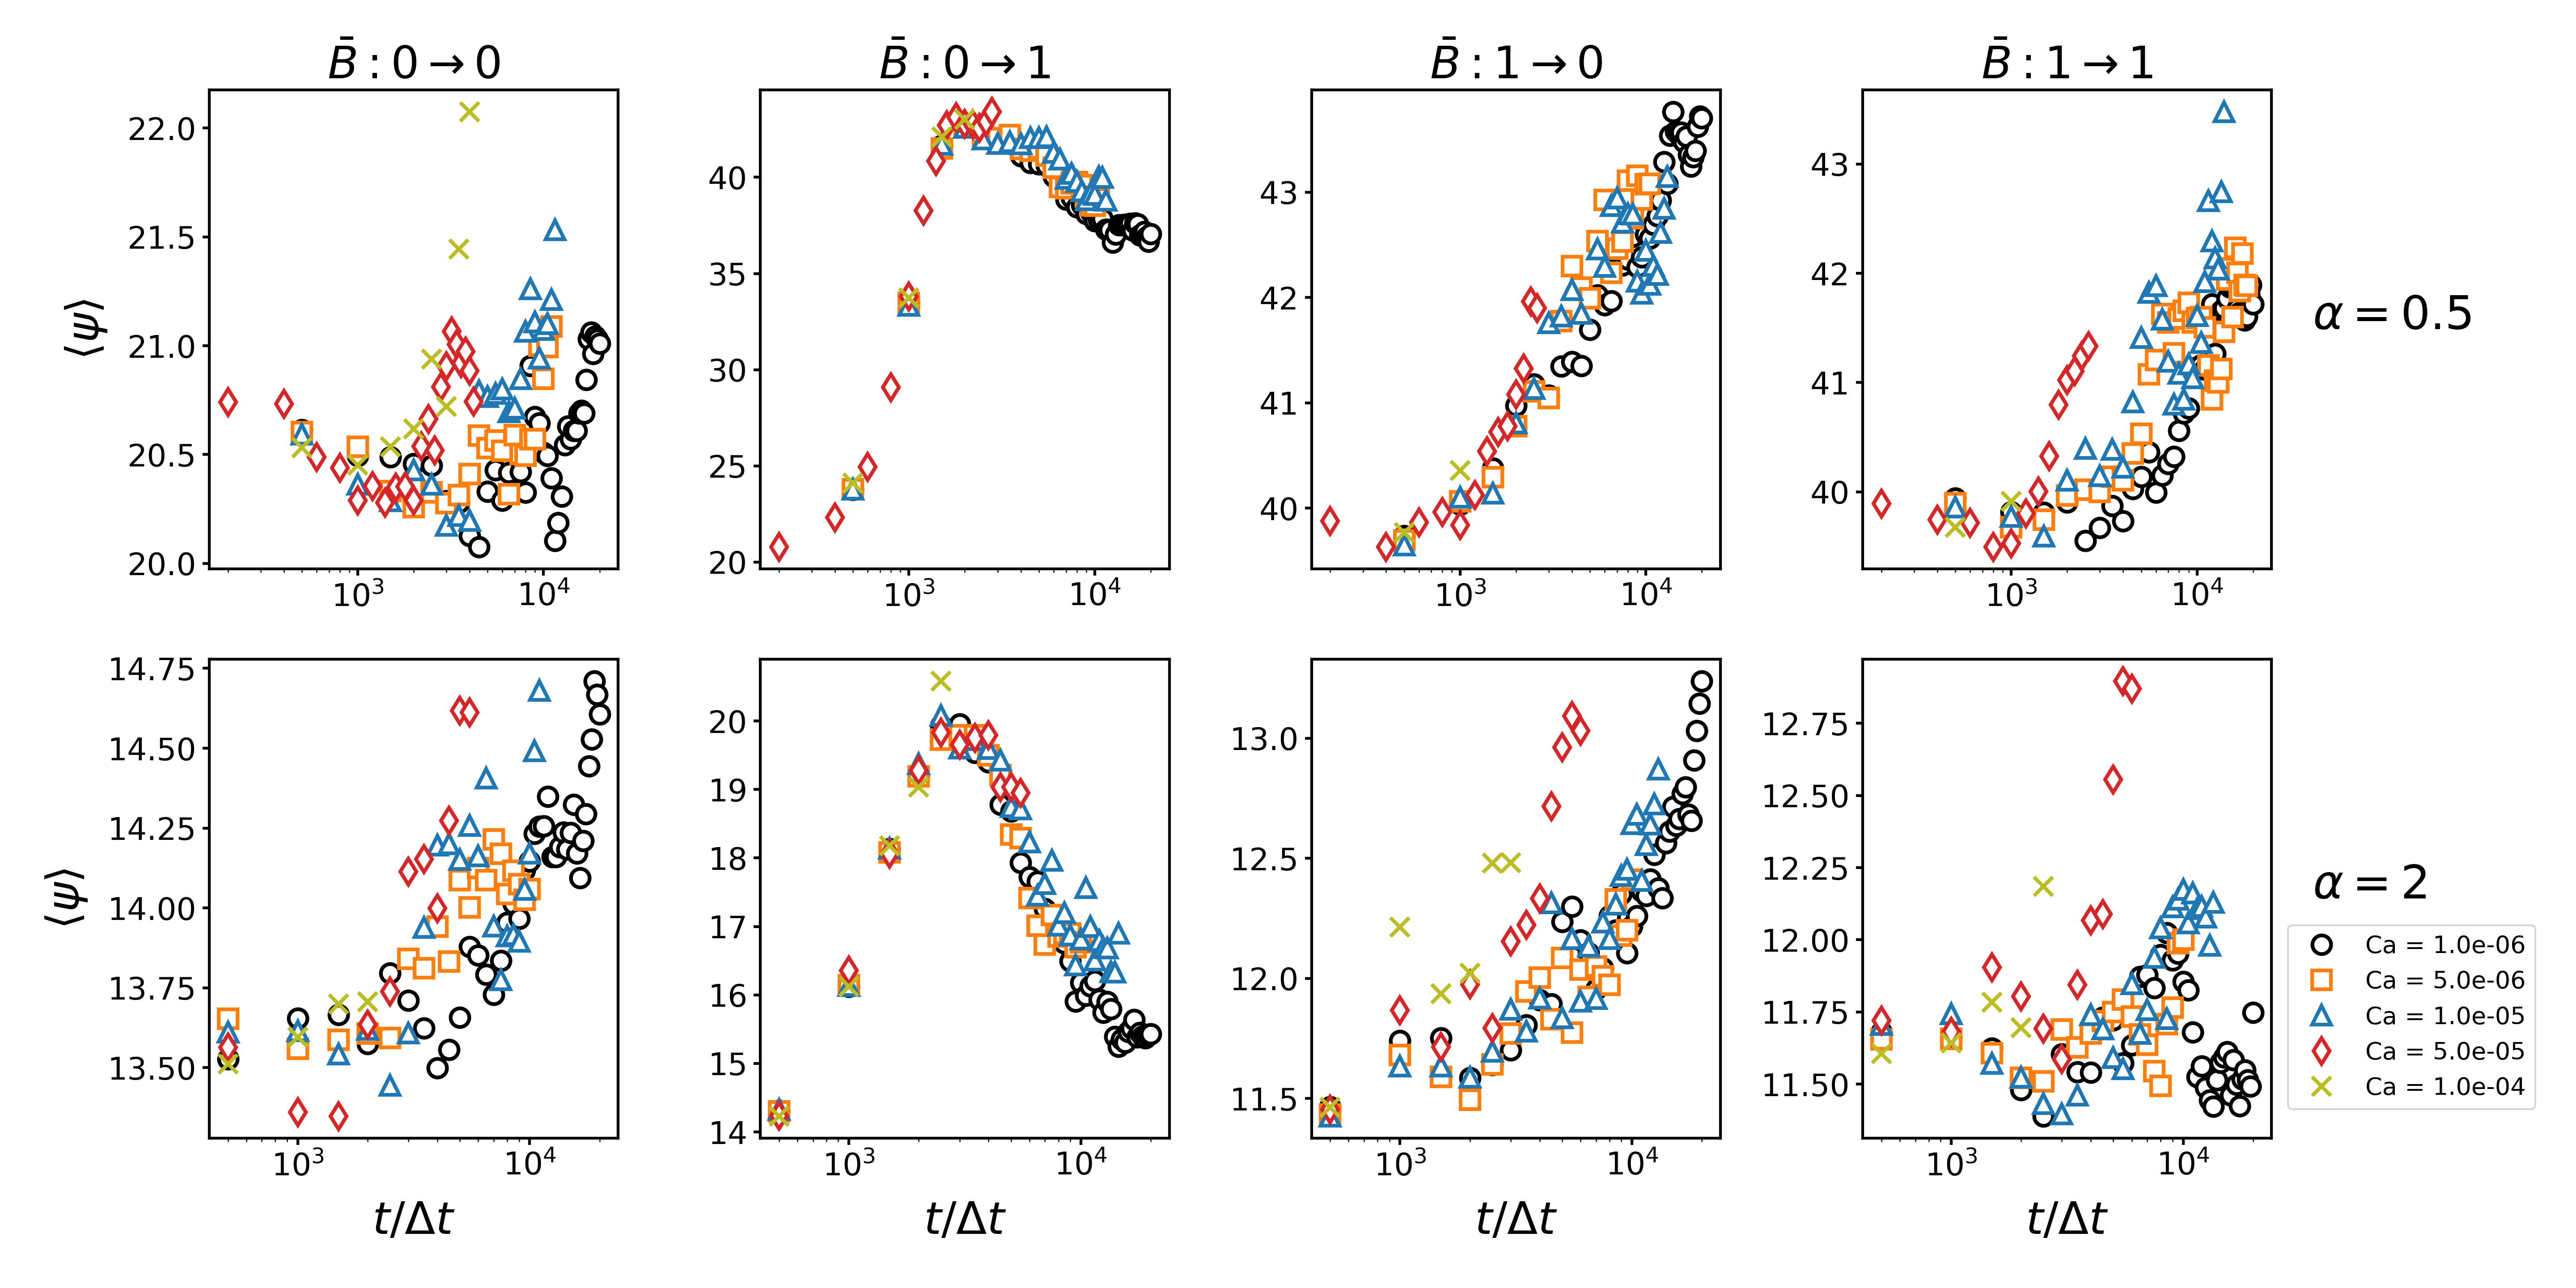
\includegraphics[scale=0.3]{../figures/results/paper3/psi-time_compare.png} 
    \caption{Comparisons of the interfacial angle of bijels stabilized by ellipsoidal particles as a function of 
             the applied shear rate at four different processing histories. We show that upon application of shear
             particles tilt out of the interface reduces the interfacial area stabilized. $\bar{B}: 0 \to 1$ shows 
             large variations in the interface angle.} 
    \label{fig:interface_angle_shear} 
\end{figure}

From Figure \ref{fig:interface_angle_shear}, we demonstrate that there is a slow increase in the interface angle over time for all cases
except for $\bar{B}: 0 \to 1$. Shear dependent $\langle \psi \rangle$ can be observed for some of the systems, indicating that the mechanism
of domain coarsening differs.The data for $\bar{B}: 0 \to 1$ is characterized as such due to a particle reorientation at the interface
in response to the field just after the magnetic field has been applied. To reduce the interfacial energy as the particles tilt from the 
interface, the interface moves with the particle until it jams in place. We can characterize the impact of the interfacial angle on the 
particle packing using the radial distribution function (rdf).

\begin{figure} 
    \centering 
    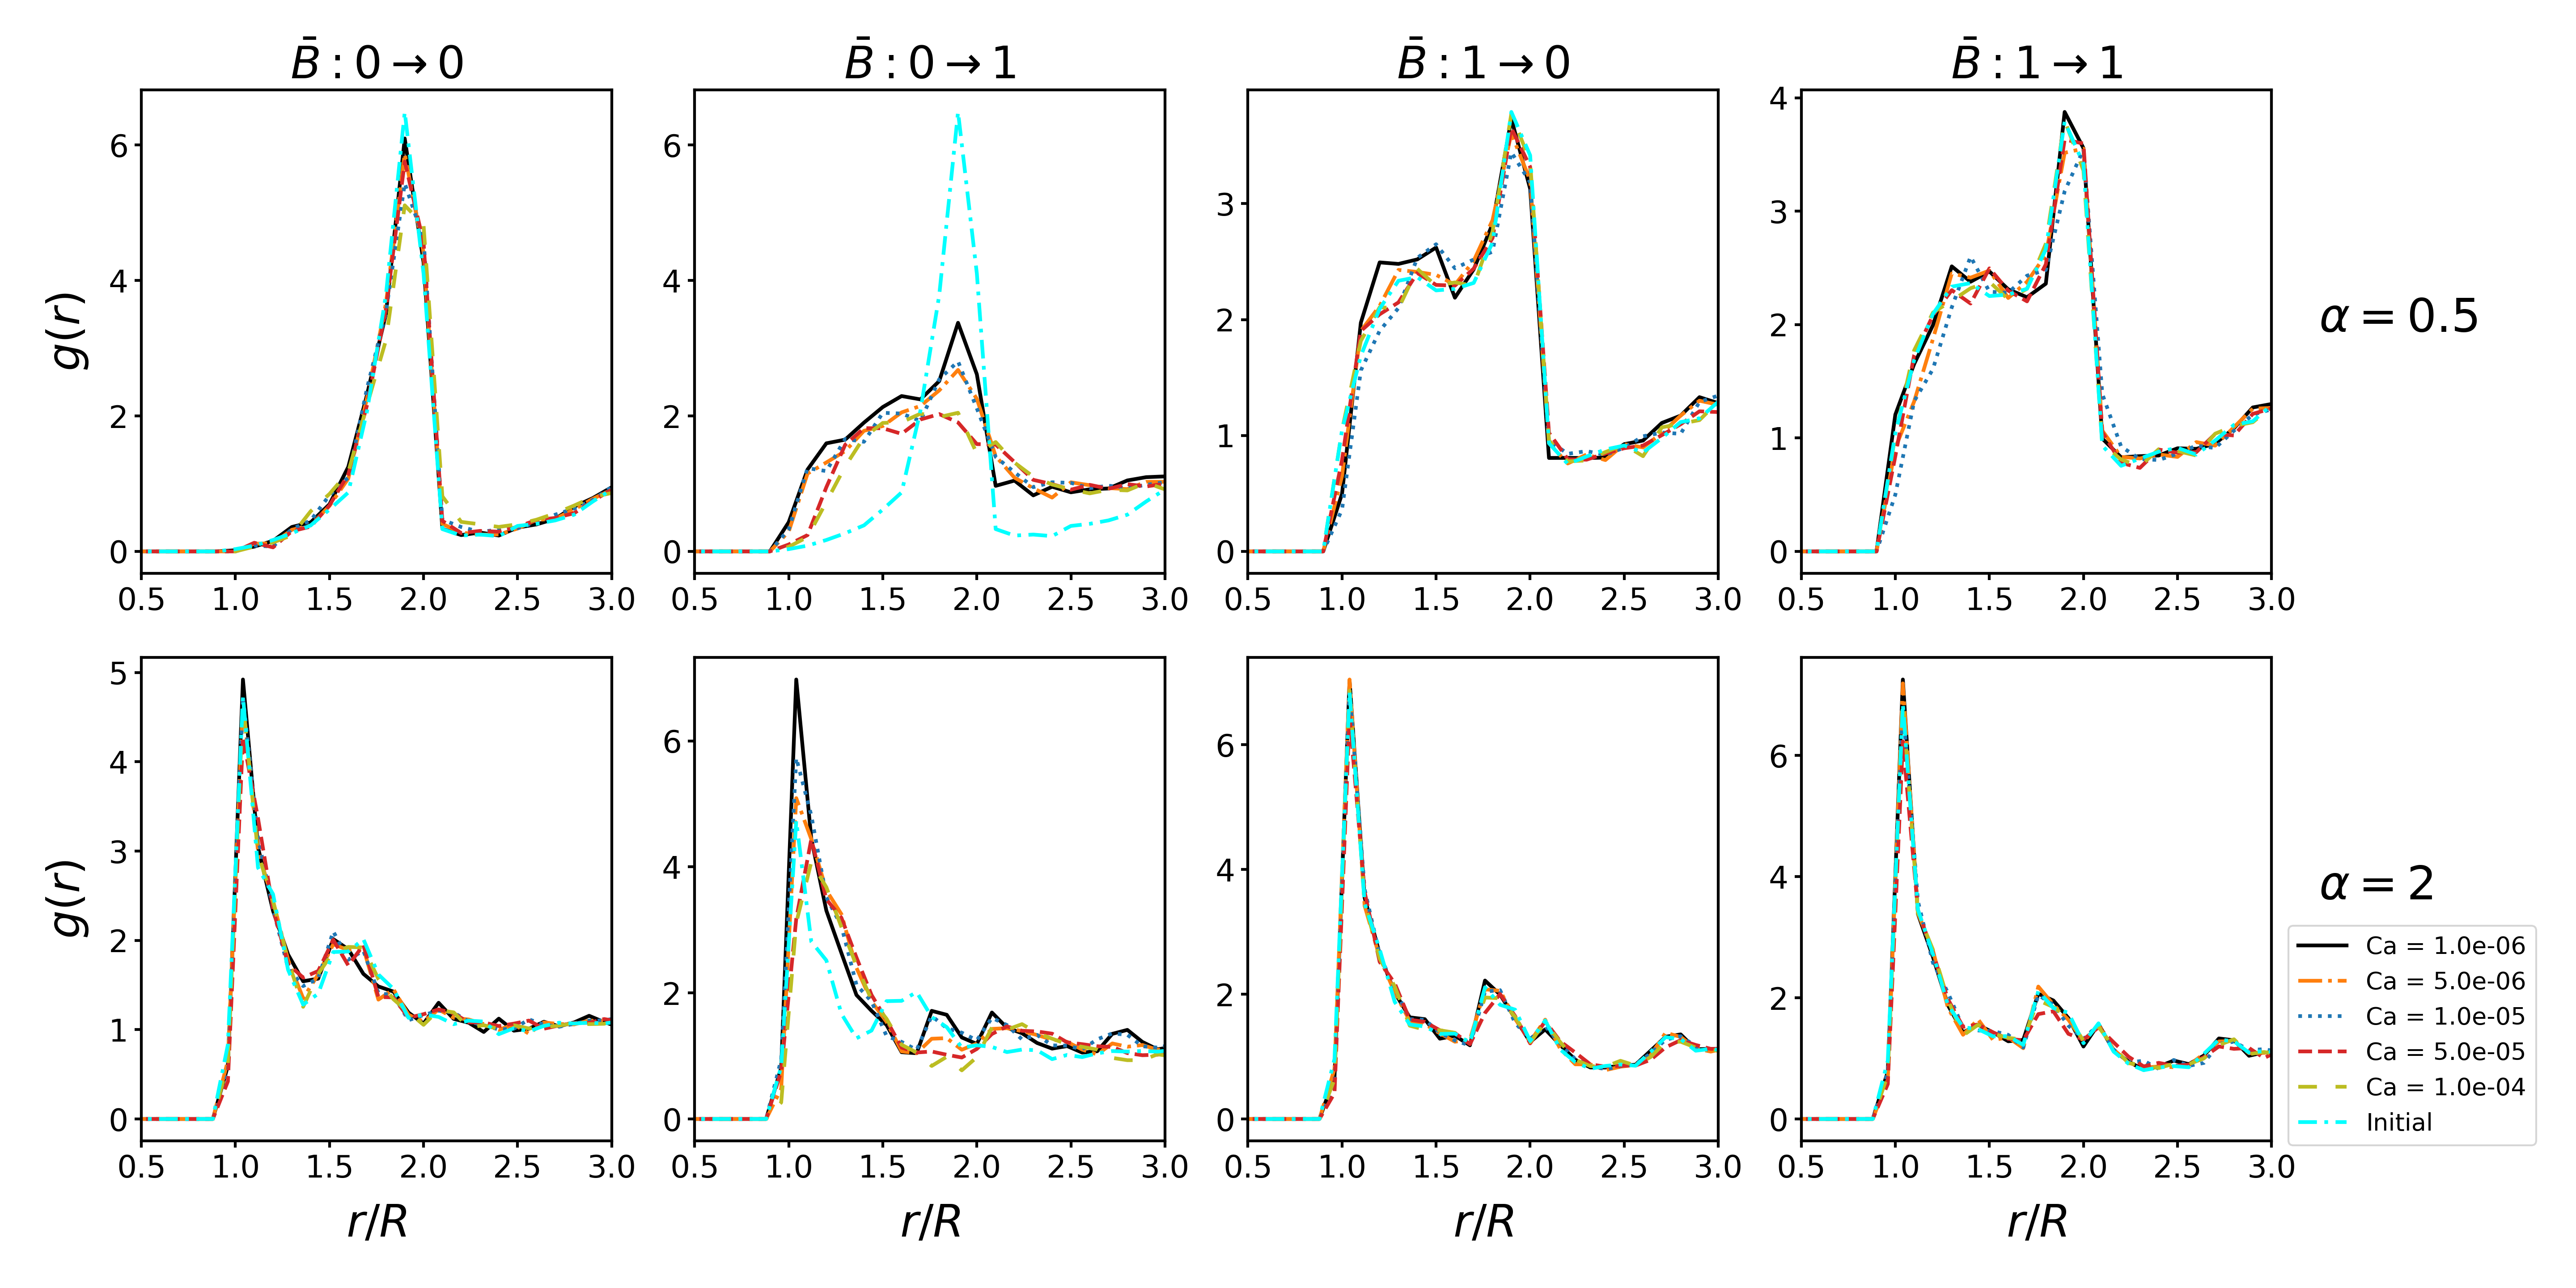
\includegraphics[scale=0.3]{../figures/results/paper3/rdf-SS.png} 
    \caption{Comparisons of the initial and final radial distribution function of the particles of bijels stabilized by ellipsoidal 
    particles as a function of the applied shear rate at four different processing histories. We show that there are minor differences
    in the particle ordering at the interface, suggesting that the particle tilting affects the coverage of particles at the interface.} 
    \label{fig:rdf_shear} 
\end{figure}

From Figure \ref{fig:rdf_shear}, we show that the change in the packing of the particles on the interface is not correlated to the change 
in the interfacial angle of the particles on the interface when changing the applied field strength in all cases. We then characterize the proportion 
of particles on the interface to investigate how the proportion of particles on the interface changes and its impact on the interfacial area.

\begin{figure} 
    \centering 
    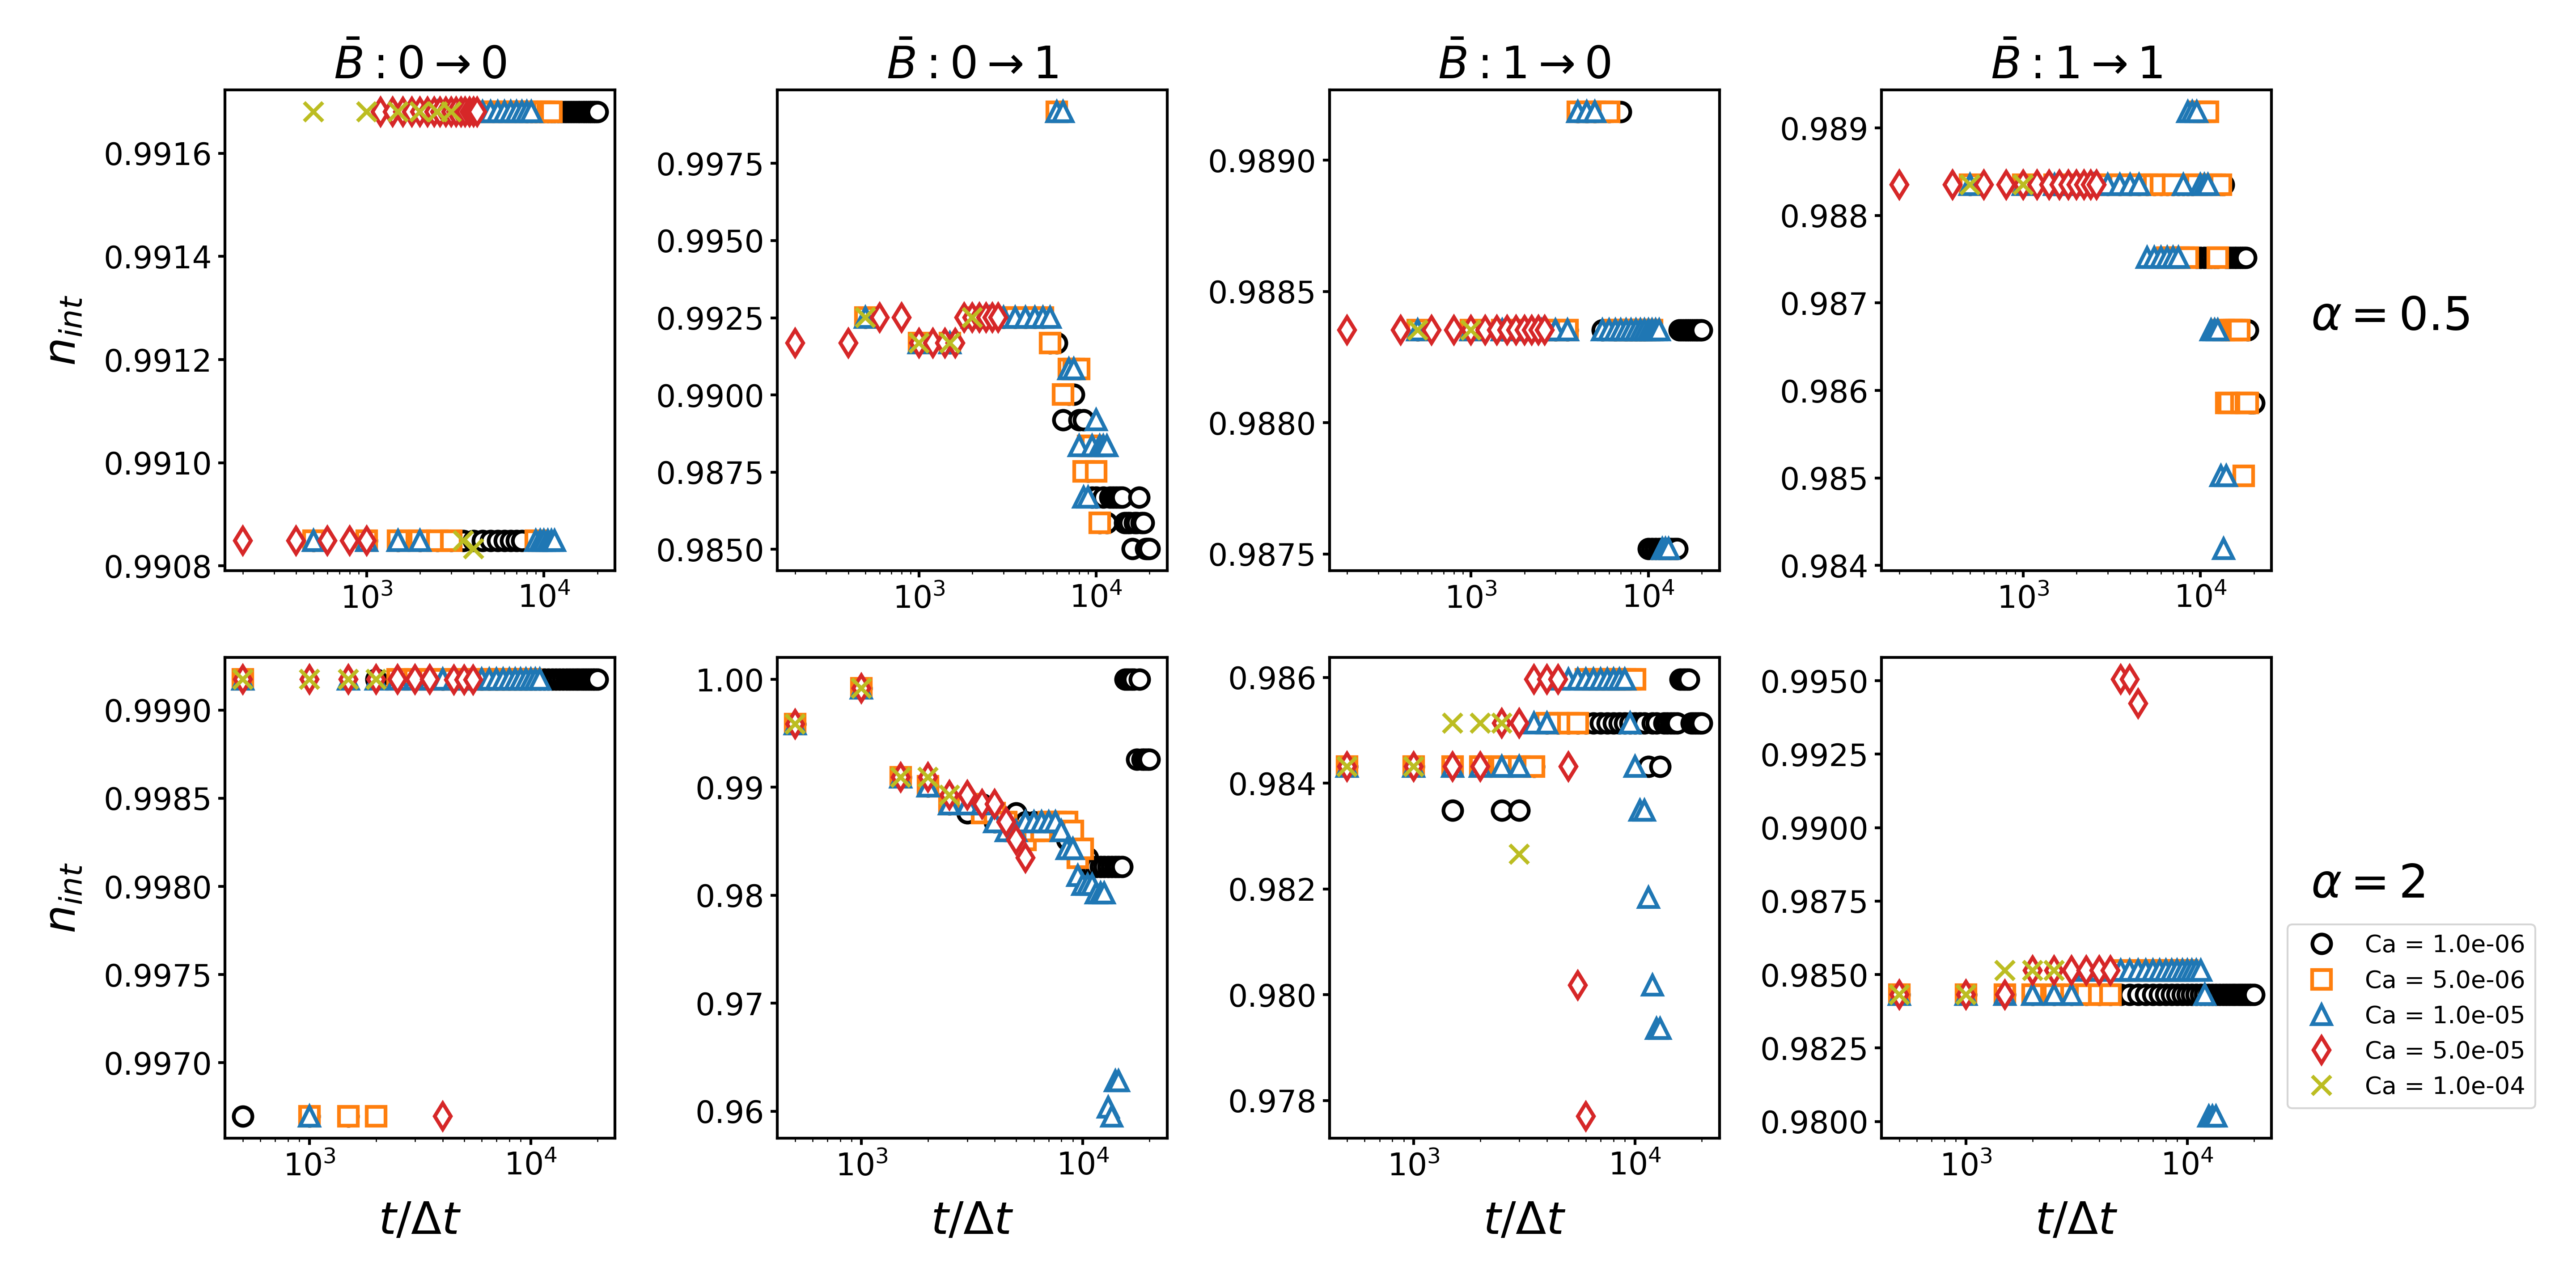
\includegraphics[scale=0.3]{../figures/results/paper3/n_int-time_compare.png} 
    \caption{Comparisons of the proportion of particles on the interface of bijels ($n_{int}$) stabilized by ellipsoidal particles as a function of 
             the applied shear rate at four different processing histories. We show that upon application of shear, many cases have a 
             reduction in the number of particles on the interface while in others it stays the same. For cases where $n_{int}$ reduces, we can 
             attribute the domain size coarsening to this effect.} 
    \label{fig:particles_interface_prop_shear} 
\end{figure}

We show in Figure \ref{fig:particles_interface_prop_shear} that when the magnetic field is kept the same between the template and during shear, the
proportion of particles on the interface ($n_{int}$) stays approximately the same. However when changing the applied field strength, $n_{int}$ more 
sensitive to shear. Here we also characterize that increasing the applied field strength reduces $n_{int}$ more than decreasing it. This is consistent
with the amount of coarsening observed for each case seen in Figure \ref{fig:domain_size_time_shear} where $\bar{B}:0 \rightarrow 1$ shows the largest
change. Next, we characterize how the microstructure and particle properties affect the constant rheology properties of the bijels.

\subsection{Viscosity measurement}

The ordering of the particles play an important role in determining the rheology of suspensions as ordered particles can slip over one another
before the structure breaks. The adsorption of particles on the interface of a bijel could affect how this slip occurs. Previous work investigating
the rheology of bijels have determined shear thinning behavior characterized with a Herschel-Buckley fit equation. We perform this analysis on the
structures we have simulated. First, we plot the shear stress over time.

\begin{figure} 
    \centering 
    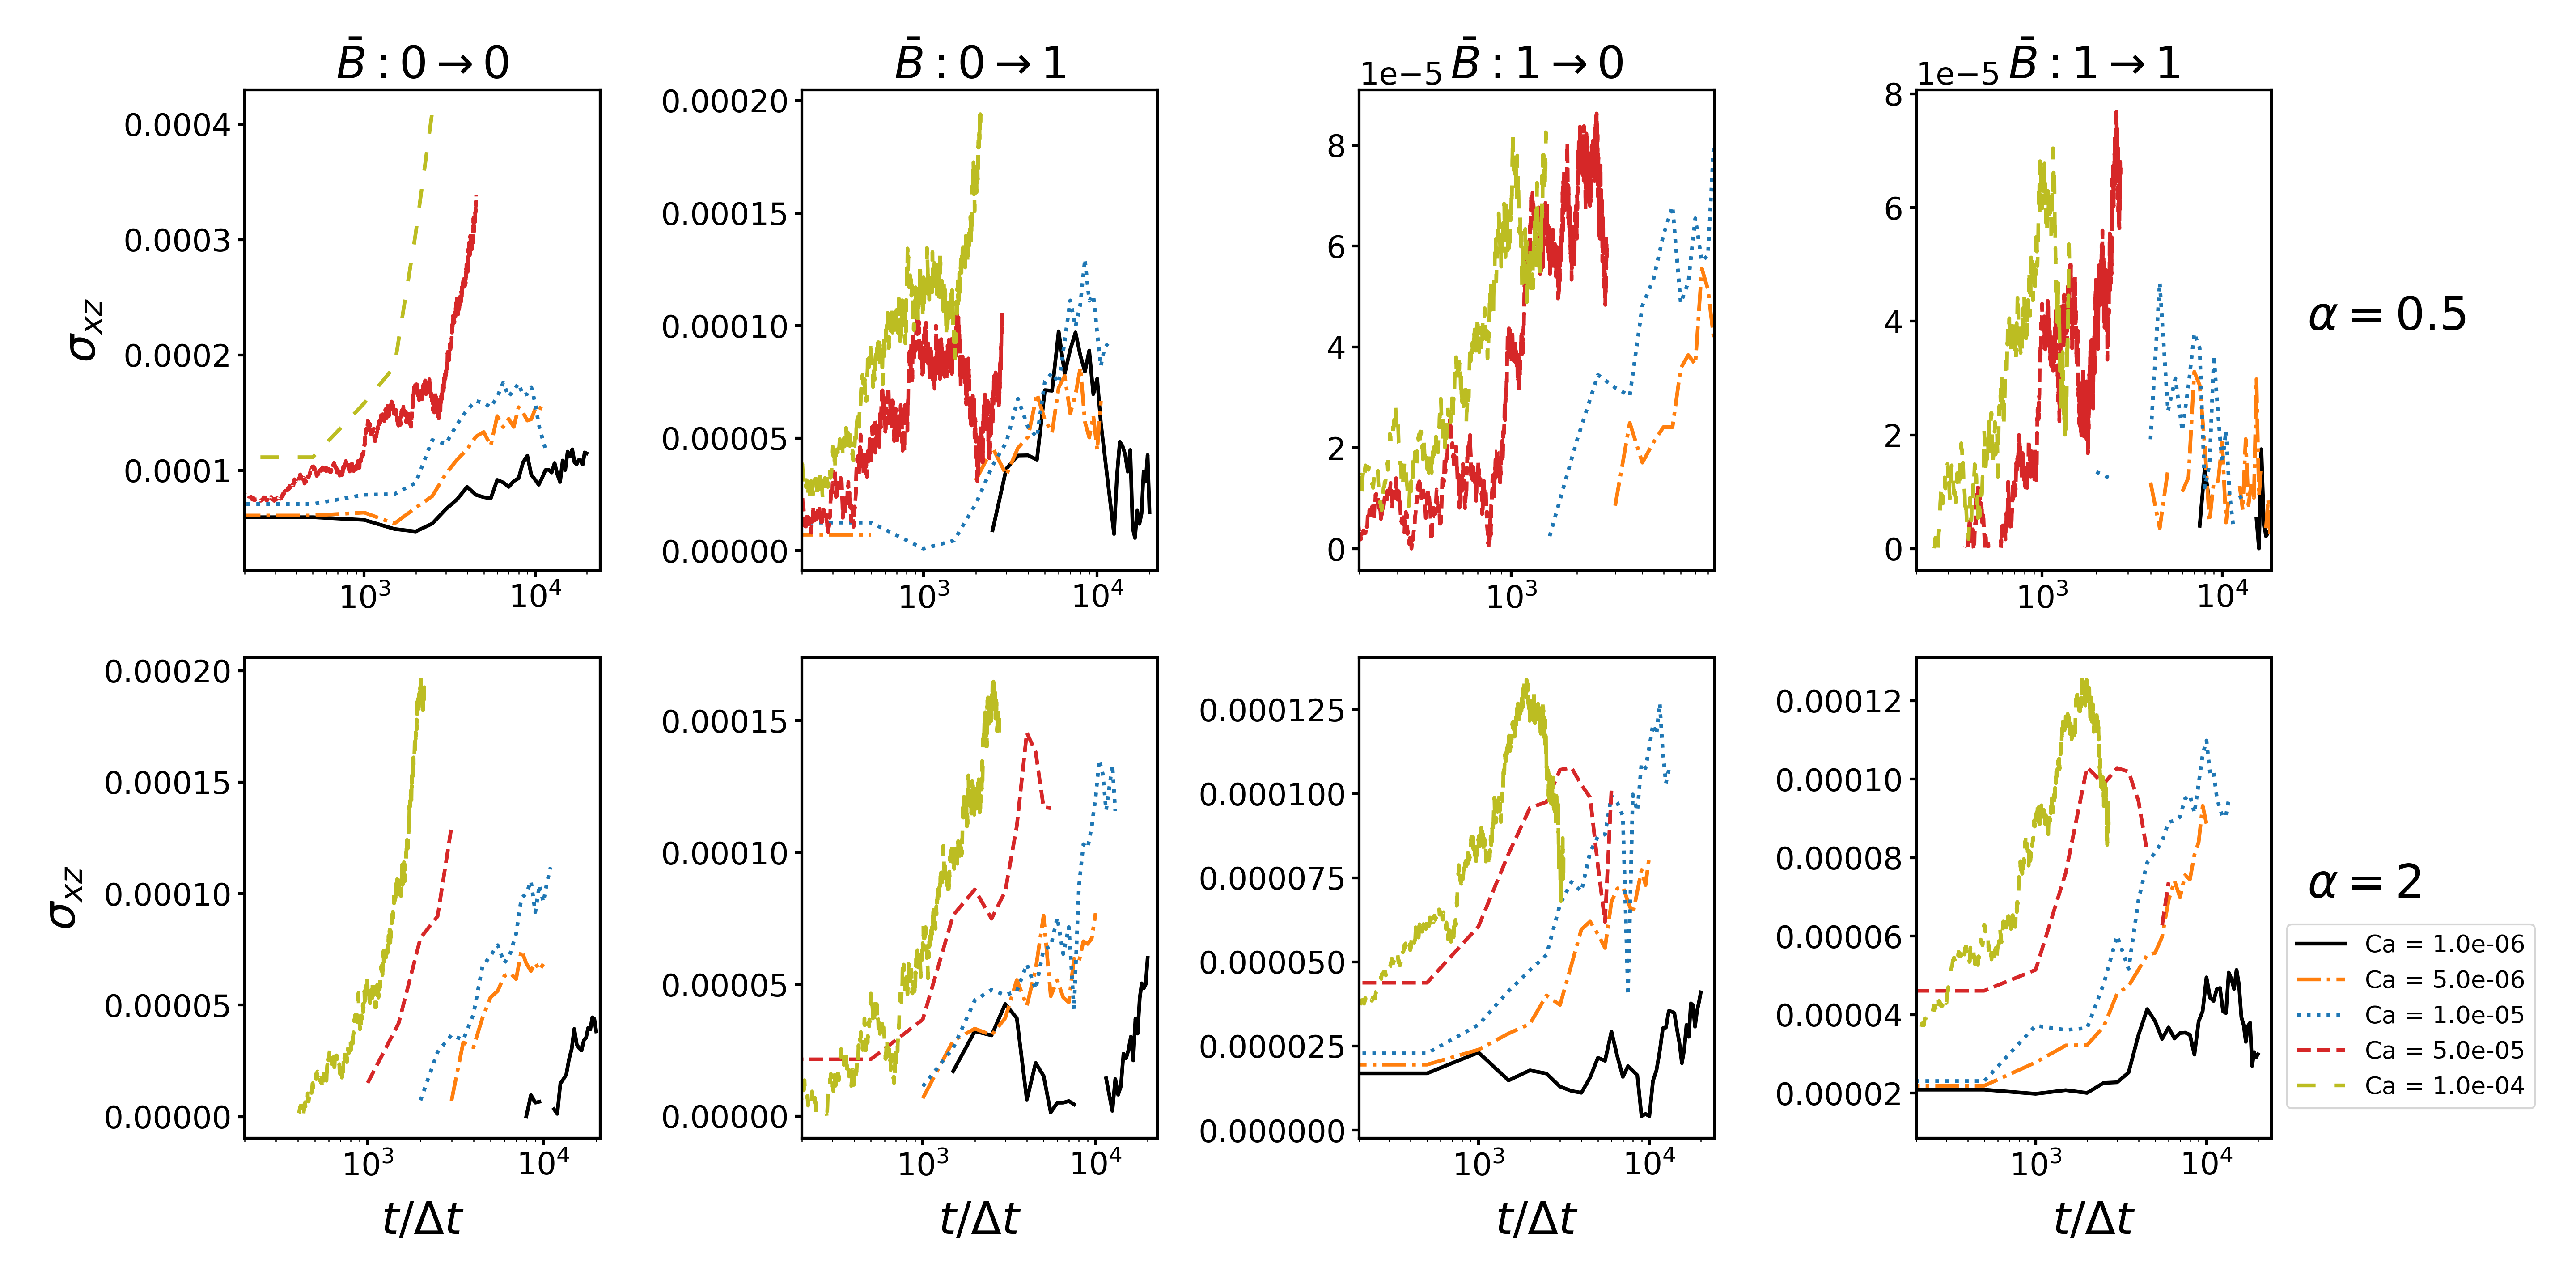
\includegraphics[scale=0.3]{../figures/results/paper3/stress-time_compare.png} 
    \caption{Time evolution of the shear stress of bijels stabilized with ellipsoidal particles as a function of the applied strain rate as
             a function of the initial microstructure and applied magnetic field. The observed stress response is difficult to say when a steady
             state is reached.} 
    \label{fig:stress_time} 
\end{figure}

Figure \ref{fig:stress_time} shows that there is no definitive steady state value of the shear stress obtained from the experiments performed. This is
attributed to the coarsening of the domains and reorientation of particles at the interface. To characterize the viscosity, we identify pseudo-steady
state regions within each of the shear stress plots and fit the stress identified within this pseudo-steady state region to the strain rate. We fit 
the stress to the strain using a Herschel-Buckley rheology model, $\sigma_{xz} = \sigma_{y} + K(\dot{\gamma})^{n}$. $\sigma_{xz}$ is the experimental
shear stress, $\sigma_{y}$ is the yield stress of the bijel, $K$ is the flow consistency index and $n$ is the flow index.
Where appropriate, we include results corresponding to a shear capillary number of $Ca_s = 10^{-6}$.

\begin{figure} 
    \centering 
    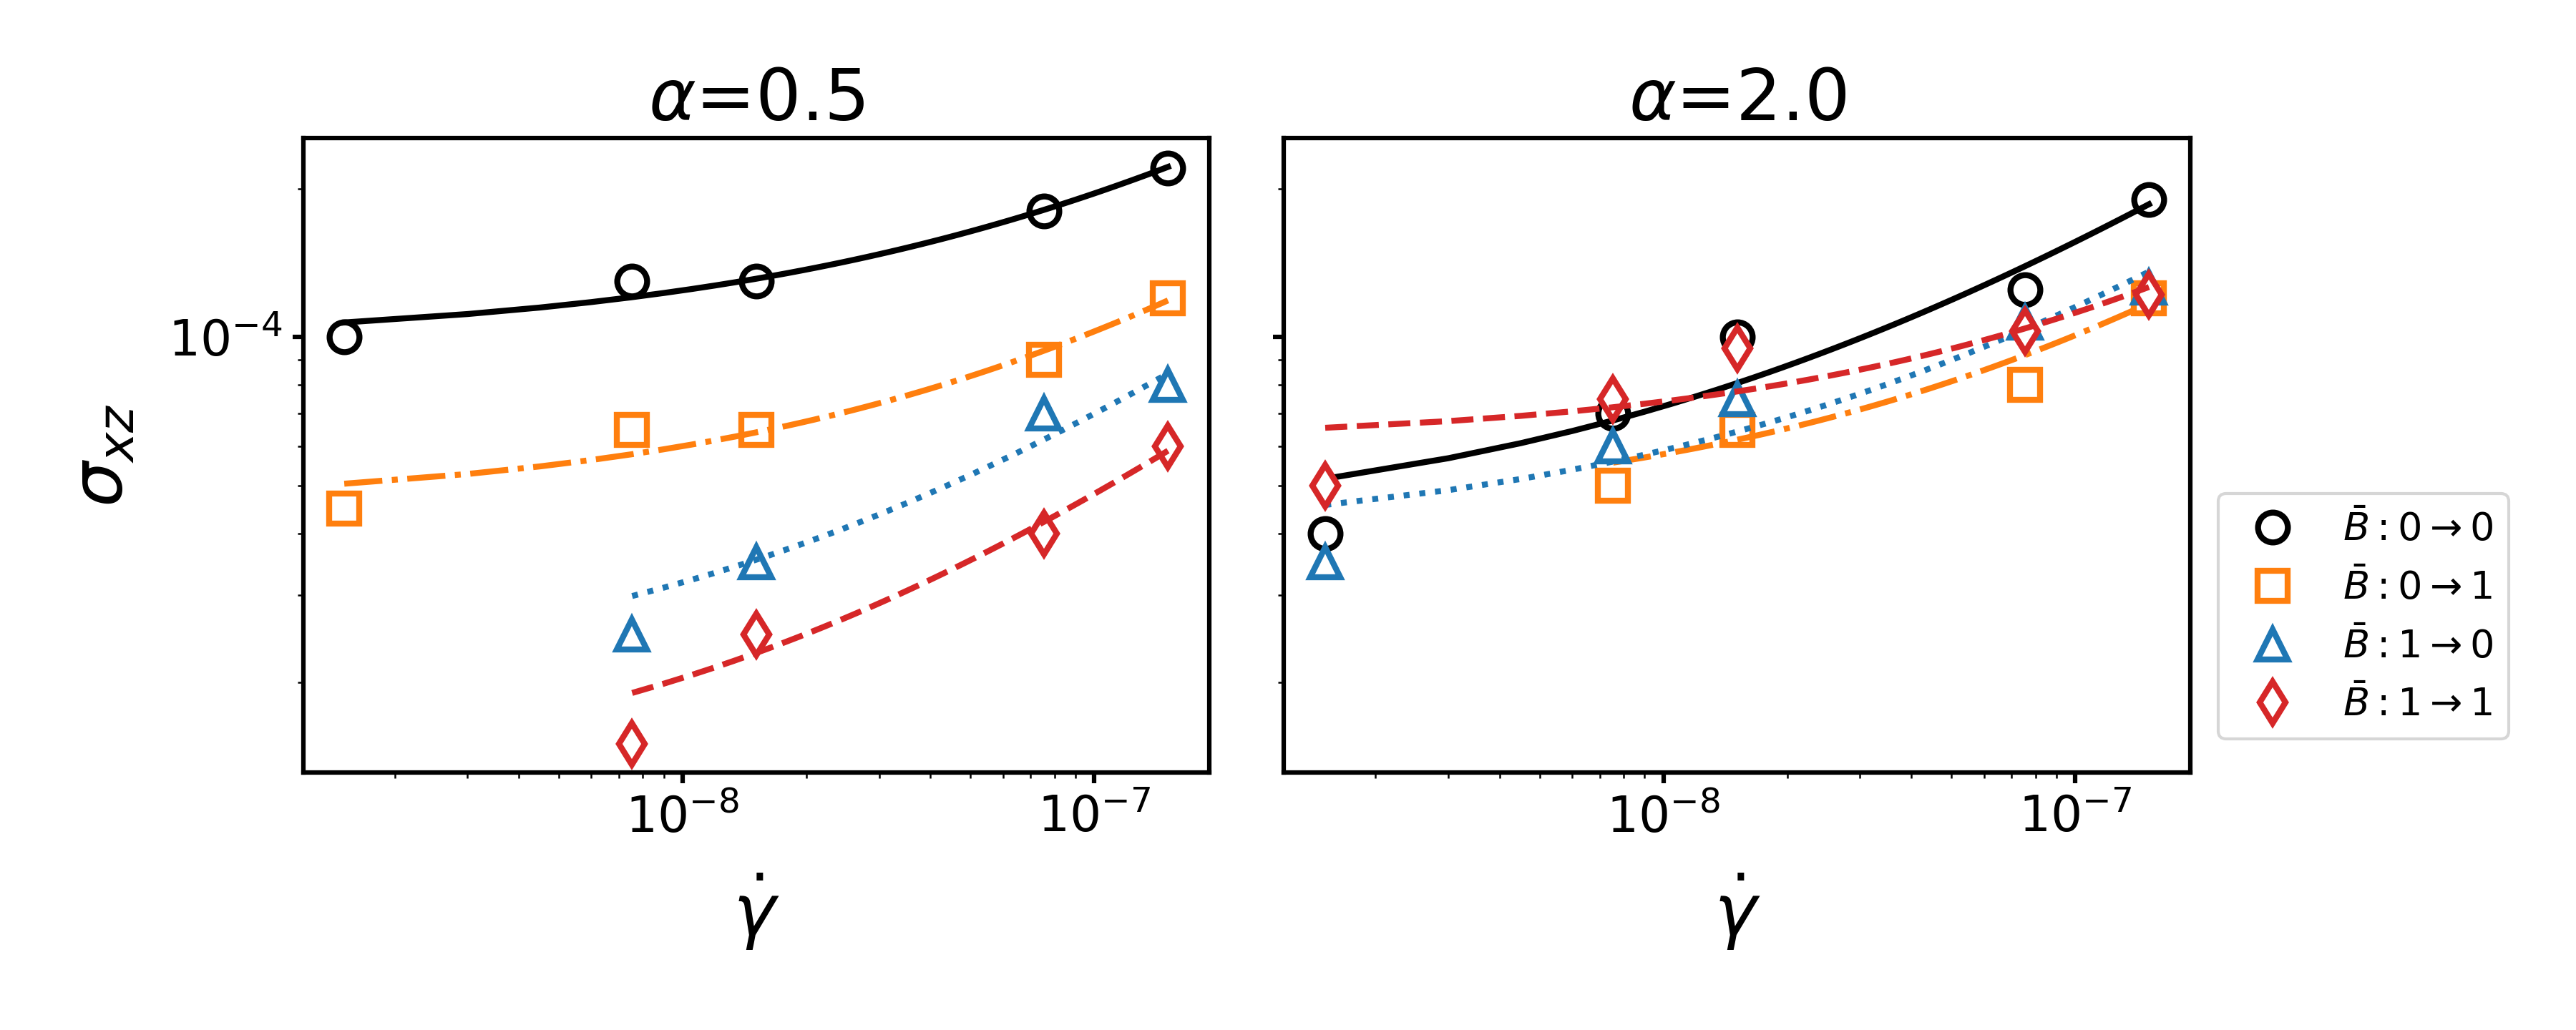
\includegraphics[scale=0.4]{../figures/results/paper3/stress_strain-all.png} 
    \caption{Fitting the experimental shear stress to the strain rate using the Herschel Buckley model. We characterize the bijels are 
             shear thinning in all cases. We show that the bijels become less shear thinning as the particle order increases. We also
             demonstrate that the particle ordering affects the yield stress differently for particles stabilized by oblate and 
             prolate particles.} 
    \label{fig:stress_strain} 
\end{figure}

From Figure \ref{fig:stress_strain}, we show that bijels stabilized with ellipsoidal particles are shear thinning regardless of the initial 
microstructure and the processing applied. We quantify the fit and tabulate the results in Table \ref{table:rheology_fit}. From Table 
\ref{table:rheology_fit}, we can see that as particle order increases, signified by an increase in the initial magnetic field, the flow index 
of the material increases, indicating more Newtonian fluid like behavior. This is due to the more ordered particles being able to slip
while undergoing fluid particle interactions without affecting other particles due to orientational ordering imposed from the application 
of magnetic fields.

\begin{table}[h!]
    \centering
    \begin{tabular}{||c c c c c||} 
     \hline
     Processing & $\alpha$ & $n$ & $K \frac{\Delta m (\Delta t)^{n-2}}{\Delta x} $ & $\sigma_{y} \frac{\Delta m}{\Delta x (\Delta t)^2}$ \\ [0.5ex] 
     \hline\hline
     $\bar{B}: 0 \rightarrow 0$ & 0.5 & 0.511 & 0.999 & $7.168 \cdot 10^{-5}$ \\ 
     \hline
     $\bar{B}: 0 \rightarrow 1$ & 0.5 & 0.579 & 0.944 & $4.008 \cdot 10^{-5}$ \\
     \hline
     $\bar{B}: 1 \rightarrow 0$ & 0.5 & 0.642 & 0.888 & $4.945 \cdot 10^{-5}$ \\
     \hline
     $\bar{B}: 1 \rightarrow 1$ & 0.5 & 0.637 & 0.914 & $1.715 \cdot 10^{-5}$ \\
     \hline
     $\bar{B}: 0 \rightarrow 0$ & 2 & 0.561 & 0.965 & $4.618 \cdot 10^{-5}$ \\
     \hline
     $\bar{B}: 0 \rightarrow 1$ & 2 & 0.609 & 0.944 & $4.101 \cdot 10^{-5}$ \\
     \hline
     $\bar{B}: 1 \rightarrow 0$ & 2 & 0.597 & 0.899 & $5.025 \cdot 10^{-5}$ \\
     \hline
     $\bar{B}: 1 \rightarrow 1$ & 2 & 0.606 & 0.885 & $6.435 \cdot 10^{-5}$ \\ [1ex] 
     \hline
    \end{tabular}
    \caption{Hershel Buckley fit parameters for different processing conditions applied to bijels stabilized by ellipsoidal particles.}
    \label{table:rheology_fit}
\end{table}
 
We characterize that the yield stress of bijels stabilized with oblate particles decrease as particle order increases while decreasing then increasing for 
prolate particles. This can be attributed to the morphology differences that lead to different interfacial packing, characterized with the rdf in Figure 
\ref{fig:rdf_shear}. We see that bijels stabilized with oblate particles do not pack as efficiently on the interface when a magnetic field is applied,
meaning that the interface can buckle more easily. In contrast prolate particles pack more densely which leads to the greater yield stress. The results
suggest that increasing the magnetic field onto bijels stabilized with prolate particles also causes the particle monolayer to more easily buckle 
upon application of shear.